\section{Project Description}
\subsection{Introduction}
%%%%%%%%%%%%%%%%%%%%%%%%%%%%%%%%%%%%%%%%%%%%%%%%%%%%%%%%%%%%%%%%%%%%%
% EHR/HAI/MDRO/what has been done and what needs to be done. 
% Part I of contribution: multi output prediction.
With the ever-growing availability of the \emph{Electronic Health Records} (EHR), many data scientists and health-informaticians have been presented with an unprecedented opportunity to improve the healthcare system by providing evidence-based solutions.  One of the costly, life-threatening but preventable problems of the healthcare system is \emph{Healthcare-Associated Infections} (HAI) which are those infections that a patient get while receiving treatment for another disease. HAIs are categorize broadly into two categories of device-associated infections (DAI) or Surgical-Site Infections (SSI). The threat of HAIs has been amplified by the recent rise of \emph{Multi-Drug Resistance Organisms} (MDRO) which makes the treatment options of the affected patients very limited. HAIs caused by MDROs are claiming tens of thousands lives every year and burden the U.S. healthcare system with around 10 billion dollars. Although there has been a lot of work for predicting the risk of each type of HAIs individually  \cite{mu2011improving, de2006surgical, friedman2007alternative, chiang2014risk, wylie2010risk, noaman2017improving, schoonover2017accurately, herc2017model, parreco2018predicting, grana2015detection, tambyah2004catheter, siddiq2012new, froon1998prediction, larsson2017risk, lisboa2008ventilator, kruger2011prognosis, mirsaeidi2009predicting} or more prevalent pathogens like Clostridium difficile (CDI) bacteria \cite{wiens2014learning, sen2017crest, oh2018generalizable, labarbera2015prediction, dubberke2011development, kuntz2016predicting}, there has been no effort in addressing the less common infections because of their scarcity. In this work, we propose to harness the recent advances in machine learning literature, specifically multi-task learning, multi-label prediction, and multi-target regression to holistically assess the patients' risk for many life-threatening MDRO-caused infections.

% Part II of contribution: hierarchy of tasks. 
Another motivation behind our proposed work stems from the fact that the severity and extent of MDRO-caused HAIs are vastly depends on the facility and the population of patients in that facilities. For example, risk prediction models developed using a dataset  from an intensive care units (ICU) can not be used directly to predict the risk of HAIs for patients in long-term care facilities. Also, since we are dealing with extremely rare events, it is not feasible to collect representative data from each facility or small care unit and develop their own predictive models from scratch. For example, although CDI cause 500,000 infections per year in U.S. hospitals, its prevalence is less than 10 percent, which leaves a 200 beds hospital with too few positive samples to build its own model for CDI risk prediction. We propose a multi-task learning framework with a tree structure task hierarchy to model the different facilities inside the hospital and to better predict the risk of various HAIs by leveraging the common and individual risk factors of patients hospitalized in different units or facilities. Furthermore, we will develop transfer learning methods for predicting risk of HAIs where patients features are not exactly equal in different facilities. 

% Part III of contribution: decision support for picking relevant intervention.
Creating risk scores and determining the risk factors for different HAIs is the limit of current risk prediction models. We want to move one step further and provide the clinicians with an ordered list of possible interventions which takes into account convenience of the patient and his/her family along with the financial cost of preventative interventions for the whole healthcare system.  {\color{red} TODO: need to expand this based on John and Courtney's inputs.}

%%%%%%%%%%%%%%%%%%%%%%%%%%%%%%%%%%%%%%%%%%%%%%%%%%%%%%%%%%%%%%%%%%%%%
% General goal beyond this dataset then more specific about this data set. 
{\bf Goal:} Our long term goal is to systematically develop prediction models which exploit data collected from multiple (heterogeneous) sources to predict different (but related) extremely rare outcomes while taking into accounts the relation between data sources and also outcomes to improve prediction accuracy of all outcomes. In this project, we plan to investigate such models toward accurate risk prediction of various extremely rare MDRO-caused HAI, in order to provide clinicians with evidence-based list of possible intervention options. The work will focus on \emph{enriching} risk prediction models with hierarchical side information about the relation of different tasks (multiple hospitals and units therein) as well as grouping of different types of HAIs (device-associated or SSI and sub-groups therein). We also build on top of the recent success of multi-label prediction and multi-target regression methods advanced by the machine learning community to simultaneously predict both the risk of developing multiple MDRO-caused HAI and also time to infections. Such predictive model will elevate our ability to better understand the risk factors involved in any of the HAIs, paving the way for accurate suggestion of preventative interventions to clinical practitioners.  

%%%%%%%%%%%%%%%%%%%%%%%%%%%%%%%%%%%%%%%%%%%%%%%%%%%%%%%%%%%%%%%%%%%%%
% What do we propose specifically? Who are working on this? What is the data set? 
{\bf Specific Objectives:} Working with a multi-disciplinary team including computer scientists, (machine learning, data mining), bioinformaticians, economists, and infectious diseases specialist, we will use the three years data of all patients admitted to the Ohio State University (OSU) hospitals which has been collected as a part of the infectious disease Learning Laboratory (LL) project ({\color{red}link to the website and; letter of support from Susan Moffatt-Bruce at the OSU hospital attached}) to develop a Machine Learning (ML) system, called DEALER, that systematically uses the extremely rare HAI-causing MDROs incidents in the pooled data from multiple hospitals and units therein, and accurately predict the temporal risk of a patient developing any of the MDRO infections during their stay at a hospital. We hypothesize that enriching our samples by merging various heterogeneous source of data along with simultaneous prediction of multiple related outcomes will both improve the prediction accuracy of all adverse events and also provides more interpretable models. In particular, our long term goal is to integrate DEALER into the OSU's patient safety learning lab called IDEA4PS whose primary goal is to improve workflows and information transfers in the healthcare environment in order to enhance patients' outcomes. Advances in both computational and statistical aspects of data analysis to be pursued in the project will be key to translating the IDEA4PS dataset into a humna-in-the-loop system that reduces adverse health events. 

%Beyond benefiting from enriched heterogeneous MDROs-caused incidents, DEALER also furthers its performance by taking into account hierarchy of hospitals, units, and wards along with their relationship with each other.

%%%%%%%%%%%%%%%%%%%%%%%%%%%%%%%%%%%%%%%%%%%%%%%%%%%%%%%%%%%%%%%%%%%%%
% What will be our contribution?
The ML system that we envision is a framework for surveillance of ``hot spots'' of HAIs which exploits electronic medical records and provides real-time risk prediction and recognizes concerning trends sooner so that clinicians can implement timely and effective interventions. Our project is motivated by a strong desire to develop methods and systems to mitigate the threat of MDROs-caused HAIs in healthcare systems. To this end, we anticipate that this project will produce the following:
\begin{itemize}
	\item It will enable accurate and timely identification of patients with high risk of developing multiple types of HAIs and provides practitioners with interpretable decisions. 
	\item It will provide smaller healthcare institutes methods to tailor mathematical HAI's risk prediction models developed for larger institutes for their environment. 
	\item It will assist clinicians in selecting proper preventative intervention which factors in patients preferences along with healthcare costs. 
\end{itemize}

%MDROs are rising (stat and image), HAI cost and death, 
%%%%%%%%%%%%%%%%%%%%%%%%%%%%%%%%%%%%%%%%%%%%%%%%%%%%%%%%%%%%%%%%%%%%%
% What has been done? What can be done to improve? 
{\bf Significance:} The United States has made significant progress toward the collective goal of eliminating HAIs, and as a result, healthcare in the U.S. is safer now than it was even 10 years ago. Building upon this success and continuing towards the elimination of HAIs is critical \cite{actionplan}. With the rise of MDROs in U.S. \cite{pop2005rising,edlin1992outbreak, whitney2000increasing} and the CDC's goal of substantially reducing multiple types of HAIs by 2020 \cite{milestones}, addressing MDROs-causing HAIs is of extreme value.  

There has been focused studies to predict patients' risk of developing infection due to the more frequent MDROs using EHRs. Clostridioides difficile (C. diff.), the most prevalent cause of HAI which sometimes become drug-resistant \cite{tenover2012antimicrobial, peng2017update, spigaglia2016recent}, has been extensively studied \cite{oh2018generalizable, wiens2012learning, wiens2014learning, wiens2012patient}.  Methicillin-resistant Staphylococcus aureus (MRSA) is the second most frequent pathogen whose risk prediction from EHR has been recently studied in isolation \cite{hartvigsen2018early, robicsek2011electronic}. Due to the scarcity of HAIs associated with other MDROs, comprehensive analysis of risk factors and risk stratification of patients for them remained unexplored. Since the distribution of frequent pathogens and their resistance pattern are changing \cite{weiner2016antimicrobial} and many of the extremely rare MDROs are more fatal than their rare counterparts \cite{resistance}, comprehensive investigation of all HAIs caused by MDROs is of extreme significance. 

%(e.g., healthcare-associated exposure, age, underlying disease, etc.), HAIs
%continue to be a signicant problem throughout the world (Klevens et al., 2007). In recent
%years there have been numerous articles citing our inability to prevent HAIs (Miller et al.,
%2011; Umscheid et al., 2011; Sievert et al., 2013).


%providing the ability to track adverse events longitudinally over the spectrum of a particular
%patient’s receipt of health services. More research on the use of electronic data for
%surveillance of HAIs is needed.


% Define terminology, data type in detail
\subsection{Scientific Background and Data Sources}

%%%%%%%%%%%%%%%%%%%%%%%%%%%%%%%%%%%%%%%%%%%%%%%%%%%%%%%%%%%%%%%%%%%%%
% What is EHR? What types of problems have been addressed? 
One of the key initiatives of the US government to decrease cost and improve healthcare quality is the mandating of health care providers to implement Electronic Health Record (EHR) systems \cite{ehr}. EHRs are real-time, patient-centered records that make information such as demographics, medications, laboratory test results, diagnosis codes, and procedures, available instantly and securely to authorized users. While the primary goal of an EHR system is electronic documentation of patients’ care, the collected data is often serve as an input source for many clinical informatics applications with the goal of extracting actionable information to improve diagnostics and patients outcomes \cite{yadav2018mining, rajkomar2018scalable, shickel2018deep}. Some of the tasks that EHR has been successfully used for include cohort identification \cite{kirby2016phekb, shivade2013review}, risk prediction \cite{ng2014paramo, wiens2012patient}, biomarker discovery \cite{bitton2010framingham}, and adverse event detection \cite{levinson2010adverse, torio2006trends}. Broadly, an adverse event is a detrimental effect of patient health as a result of medical care. The goal of our proposed work is to predict a specific adverse event, namely rare infections using EHR. 

%, intervention's effect quantification

%%%%%%%%%%%%%%%%%%%%%%%%%%%%%%%%%%%%%%%%%%%%%%%%%%%%%%%%%%%%%%%%%%%%%
% What is HAI? Why is it important to address?(Cost and Occurrence)
\emph{Hospital-Acquired Infection} (HAI) or more broadly healthcare-associated infection is an infection a person get while he/she is receiving health care for another condition. Although often being preventable \cite{progress, yokoe2014compendium, umscheid2011estimating}, HAIs have been the cause of many diseases and deaths among hospitalized patients \cite{miller2011comparison, cdc, scott2009direct, klevens2007estimating} and their elimination is a priority of the Department of Health and Human Services \cite{hhs}. It is estimated that at any given time, about 1 in 25 inpatients have HAI \cite{magill2014multistate, hhs}. Other studies report the estimated number of HAI associated death to be around 99000 per year \cite{klevens2007estimating} while burdening the U.S. healthcare budget by \$5 to \$10 billion annually \cite{stone2005economic, zimlichman2013health}, Figure \ref{money}. 

\begin{figure}
	\centering
	\subcaptionbox{
		Per case cost.
		\label{bar}
	}{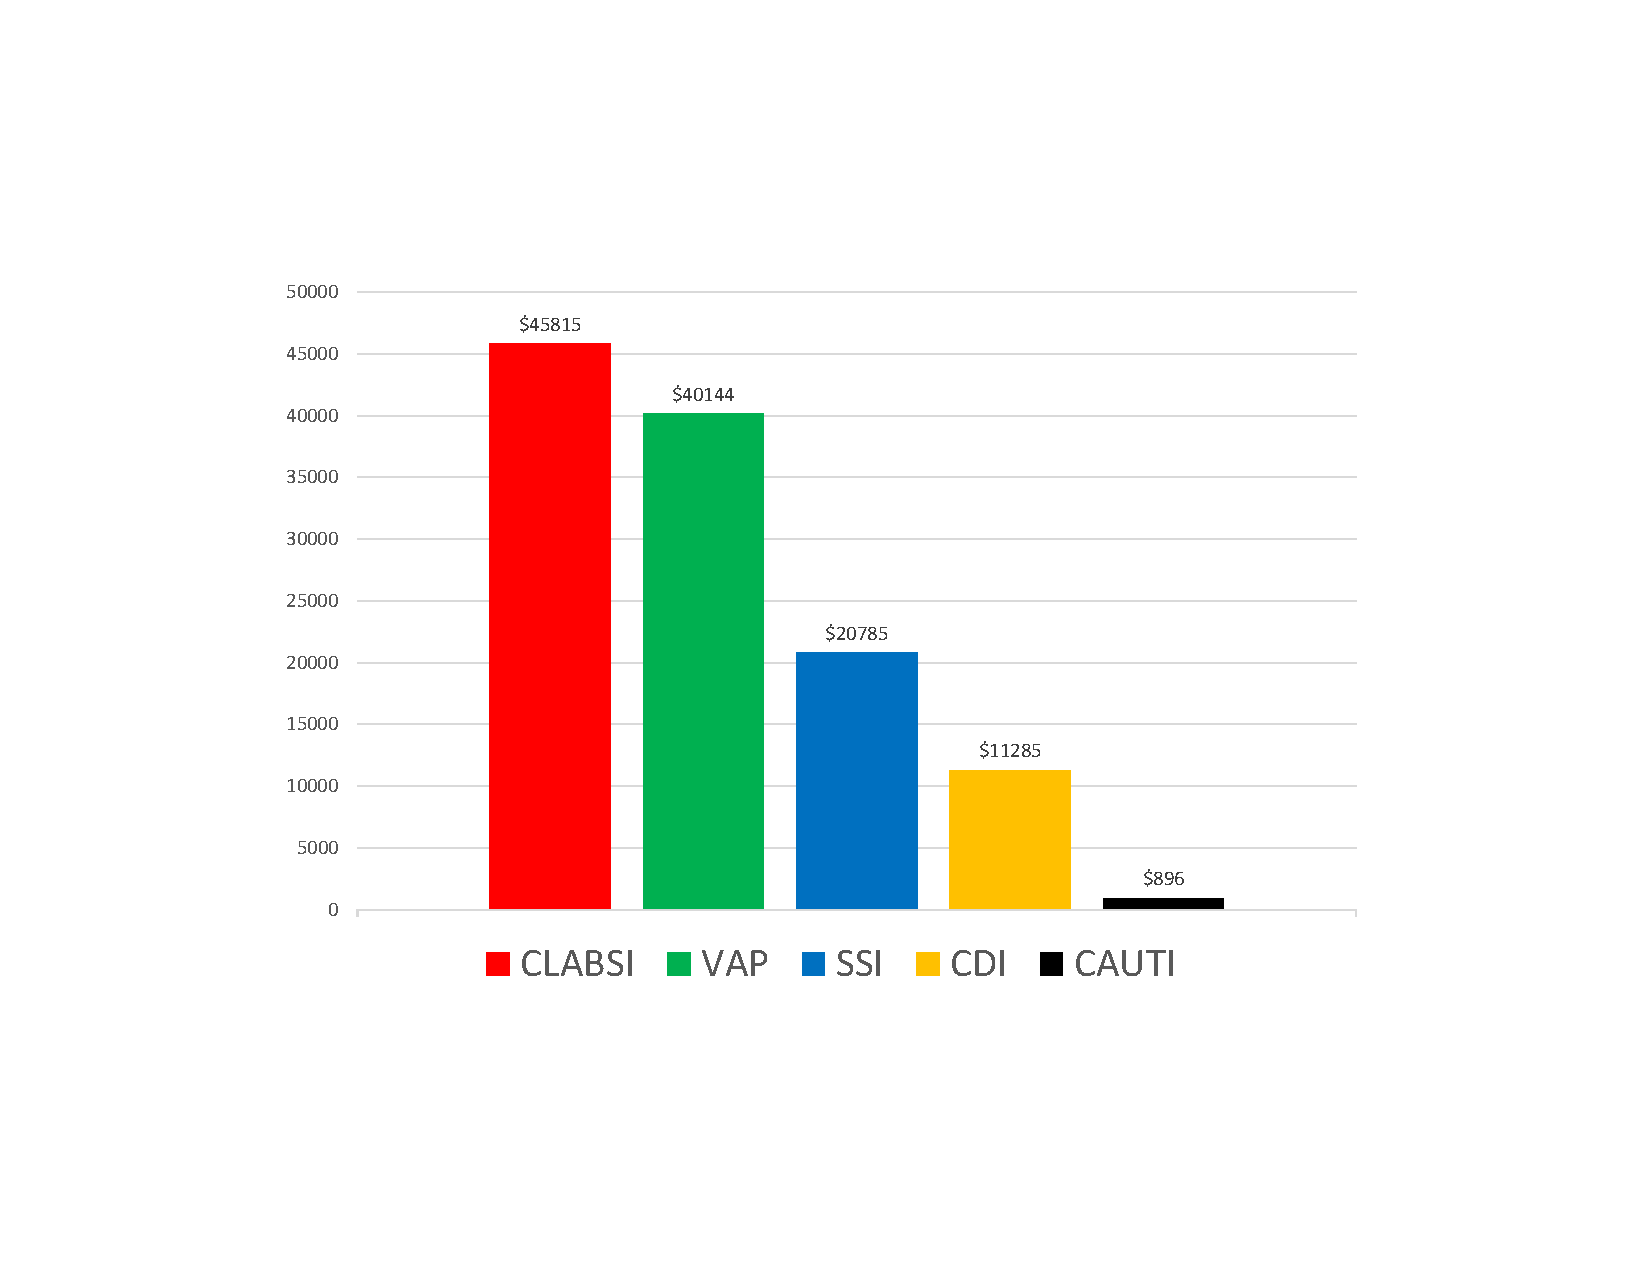
\includegraphics[width=0.35 \textwidth,]{./img/bar1}}~
	\subcaptionbox{
		Contribution percentage.
		\label{pie}
	}{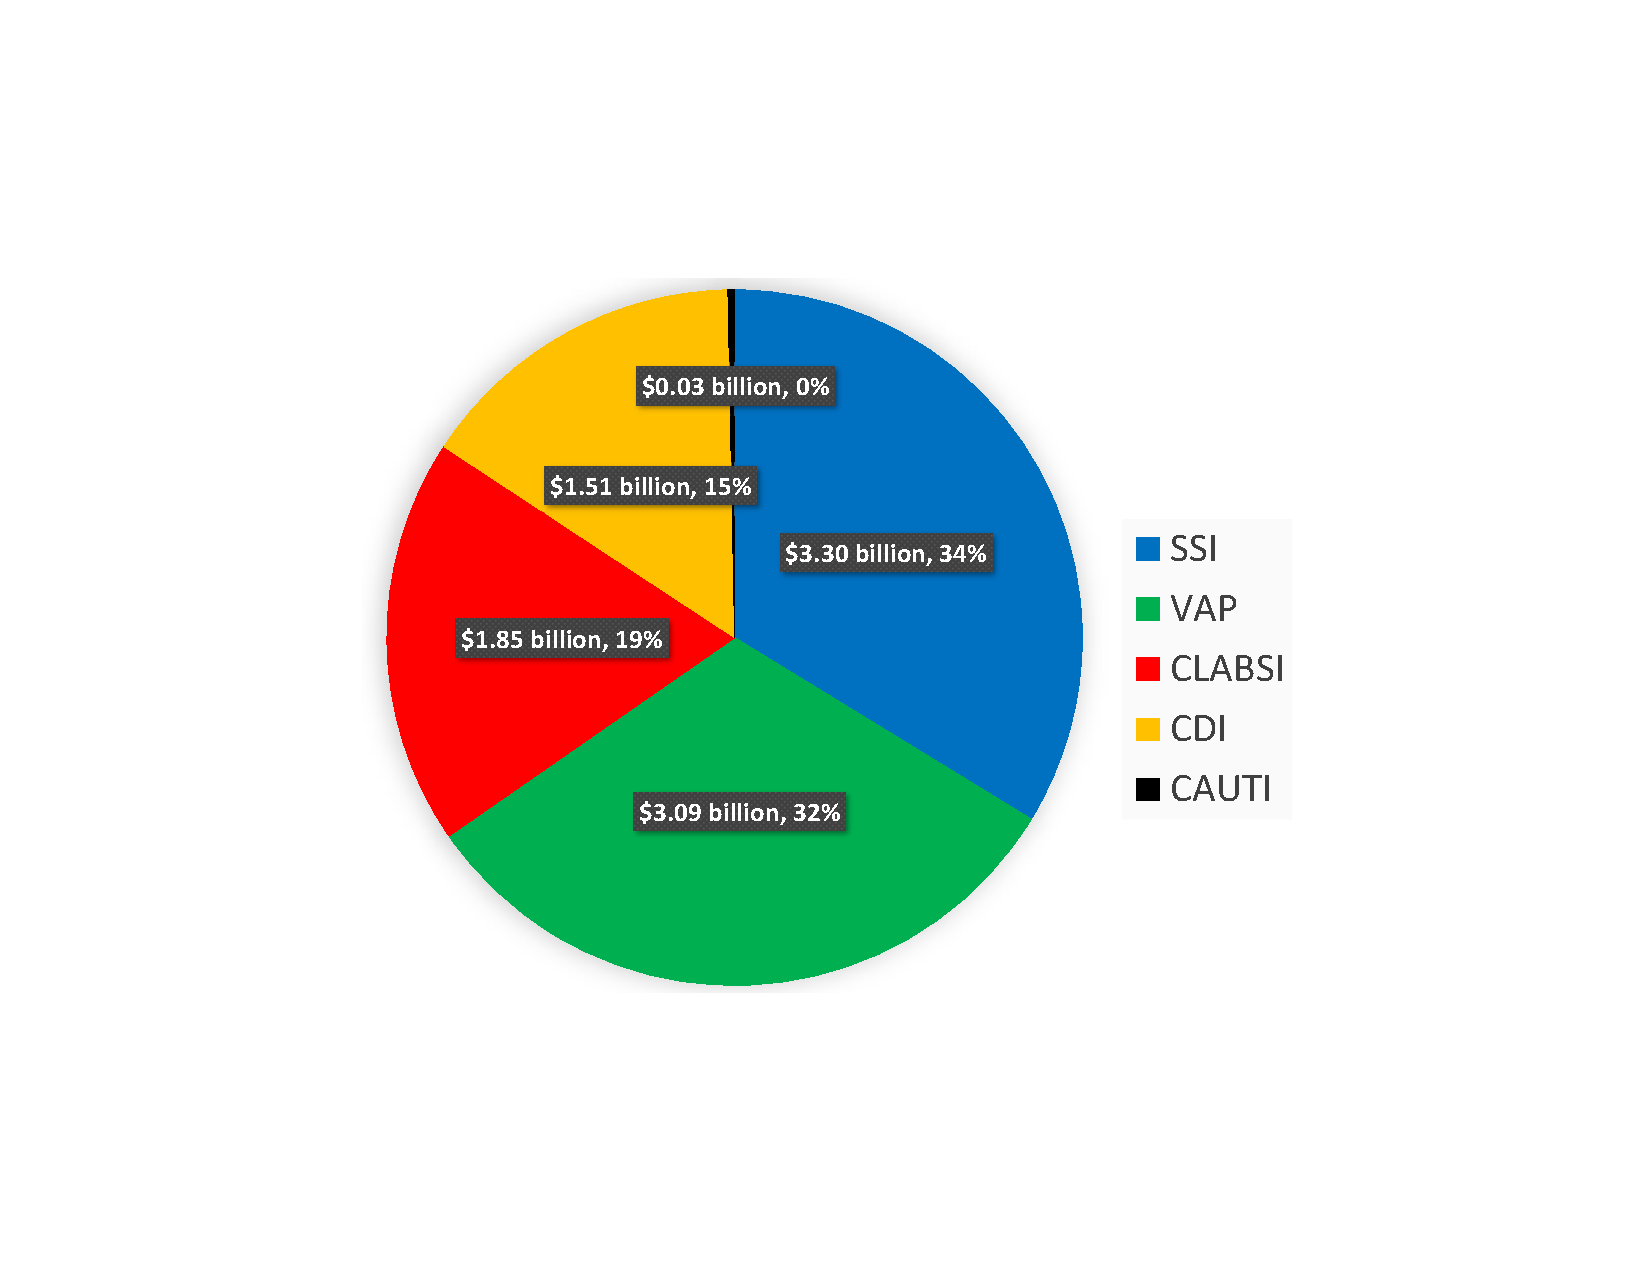
\includegraphics[width=0.3 \textwidth]{./img/pie1}}
	\caption{Cost of the five most common HAIs in the U.S. reaches the total of \$9.8 billion annually. Data source from \cite{zimlichman2013health} and figures from \cite{center}.}
	\label{money}
\end{figure}

%Approximately one-third of HAIs are preventable \cite{}.

\begin{figure}
	\centering
	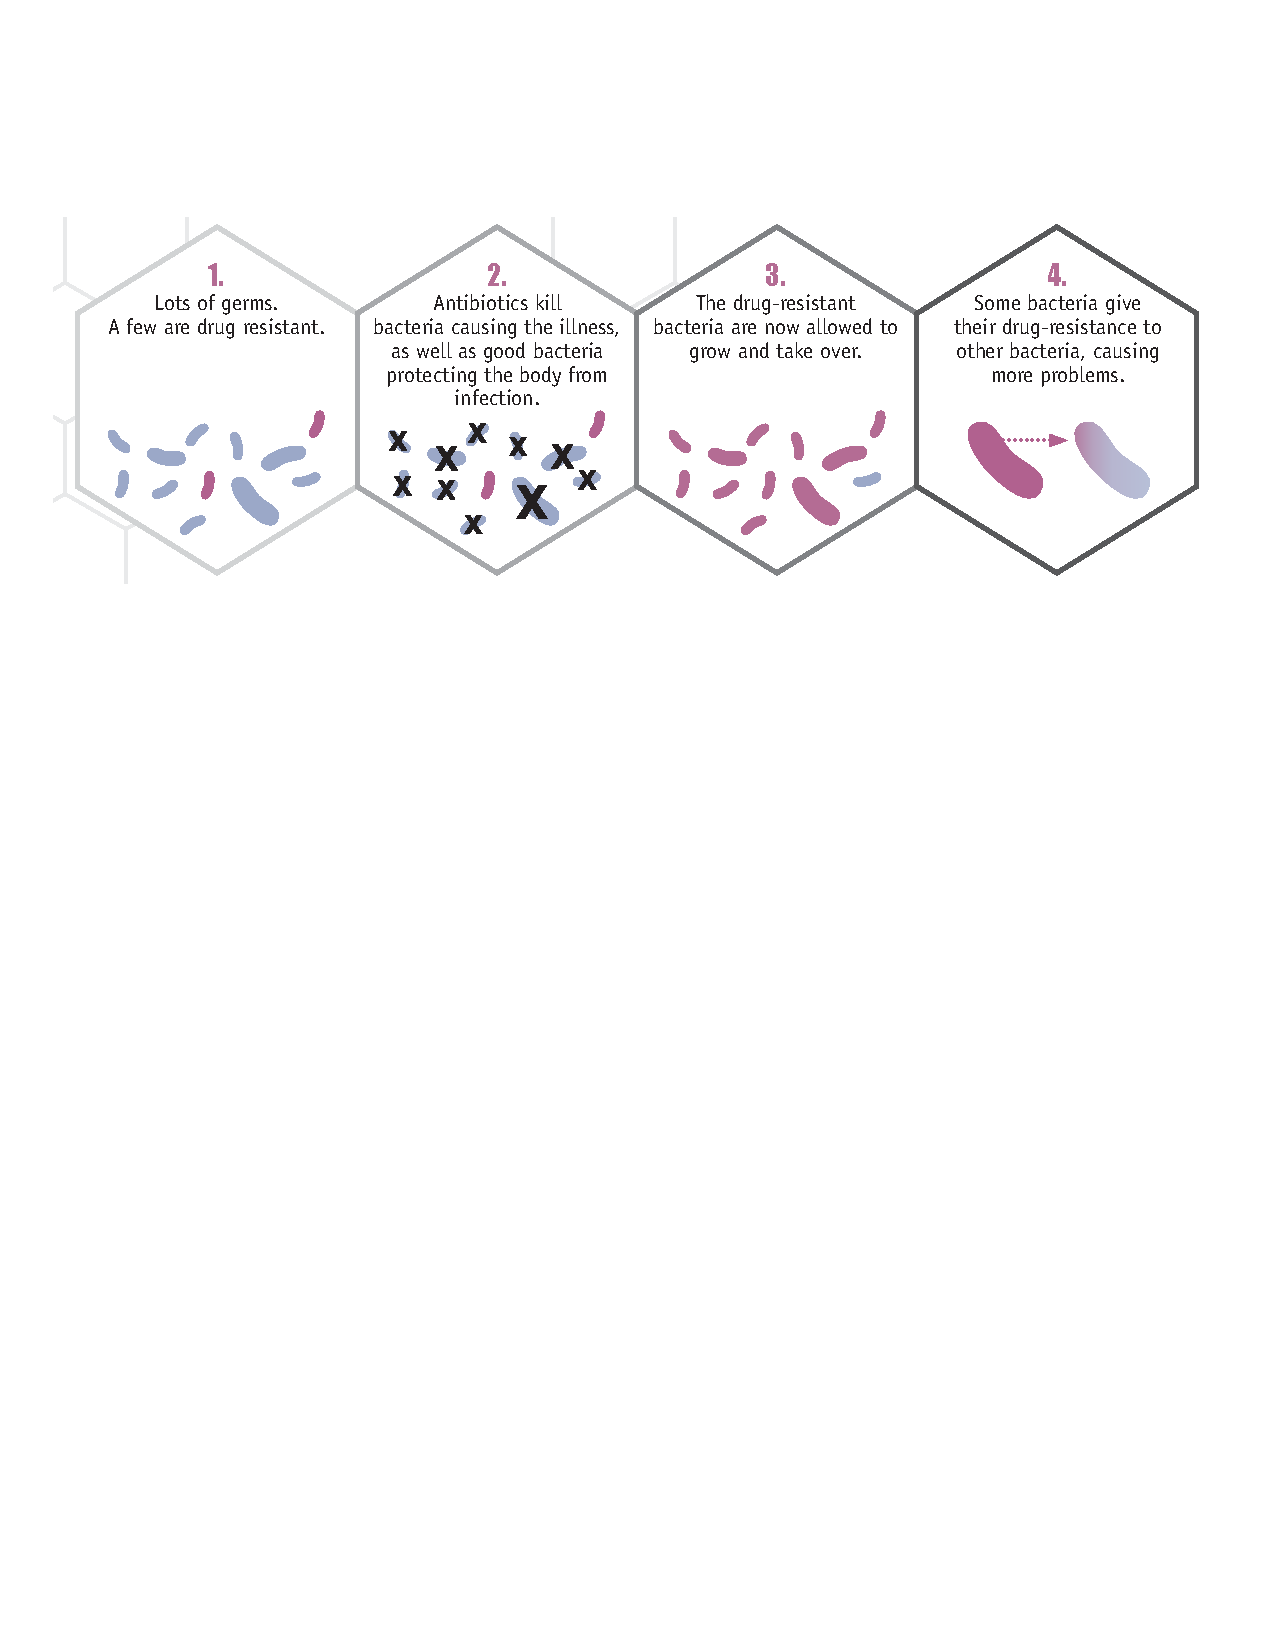
\includegraphics[width=.7\textwidth]{./img/evol.pdf}
	\caption{Antibiotic resistance as an outcome of antibiotic overuse and natural selection \cite{resistance}.}
	\label{evol}
\end{figure}



%which costs the US healthcare system ? dolloars annually and burden .
%The Centers for Disease Control and Prevention (CDC) in 2007 estimated that 1.7 million health care–associated infections incidents in over U.S. per year. A more recent estimate of HAIs in 2011 suggests that more than 700,000 infections per year burdens U.S. acute care hospitals and indicates that on any given day approximately 1 of every 25 inpatients in U.S. acute care hospitals has at least one health care–associated infection \cite{magill2014multistate} .

%%%%%%%%%%%%%%%%%%%%%%%%%%%%%%%%%%%%%%%%%%%%%%%%%%%%%%%%%%%%%%%%%%%%%
% What are MDROs? Why are they important?
Though the rate of many HAI types have dropped over the last decade \cite{progress} increasing trends in prevalence rates of HAIs caused by \emph{Multi-Drug Resistant Organisms} (MDRO) has been observed \cite{balkhair2014epidemiology, actionplan}. MDROs are pathogens, predominantly bacteria, that have the ability to defeat many of the known antibiotics, and therefore infections caused by MDROs are difficult or sometimes impossible to treat \cite{siegel2007management}. The prevention and control of MDROs is a national priority \cite{lederberg1998antimicrobial, shlaes1997society}. MDROs may naturally exists in the population of bacteria like gut microbiom without any adverse health effect, but when antibiotics kill other types of organisms in the population, MDROs take over all of the resources and produce offsprings that results in a generation of organisms all resistant to antibiotics. Finally, MDROs may amplify their presence in a population by pass their resistant-causing genetic materials to other bacteria \cite{resistance}. The process of MDRO growth due to the evolutionary pressure is depicted in Figure \ref{evol}.

%{\bf Multi-drug resistant organism (MDRO) infection:} An infection caused by a microorganism, predominantly bacteria, that is resistant to multiple classes of antimicrobials. In some cases, the bacteria have become so resistant that no available antibiotics are effective against them. In most instances, MDRO infections have clinical manifestations that are similar to infections caused by susceptible pathogens. However, options for treating patients with these infections are often extremely limited 

Multi-drug resistance has been prevailed over the last decade due to overuse of antibiotics in different settings, e.g., food animal production \cite{landers2012review}. One of the main places that hosts many MDROs are healthcare facilities, Figure \ref{resistant}. Although transmission of MDROs is most frequently documented in acute care facilities, all healthcare settings are affected by the emergence and transmission of antimicrobial-resistant microbes. It should be noted that, the severity and extent of disease caused by MDROs varies by the population(s) affected and by the institution(s) in which they are found. For example, risk of patients in institutions with varying physical and functional characteristics, like long-term care facilities, intensive care units (ICU), burn units, neonatal ICUs are varying a lot \cite{siegel2007management}. Therefore one can not build a risk prediction model for an MDRO using data from one population and transfer the built model to another facility and use it for another population of patients without suffering from prediction loss \cite{wiens2014study}. Because of this, any risk prediction model of these pathogens need to be tailored to the specific needs of each population and individual institution \cite{siegel2007management, wiens2014study}. 

\begin{figure}
	\centering
	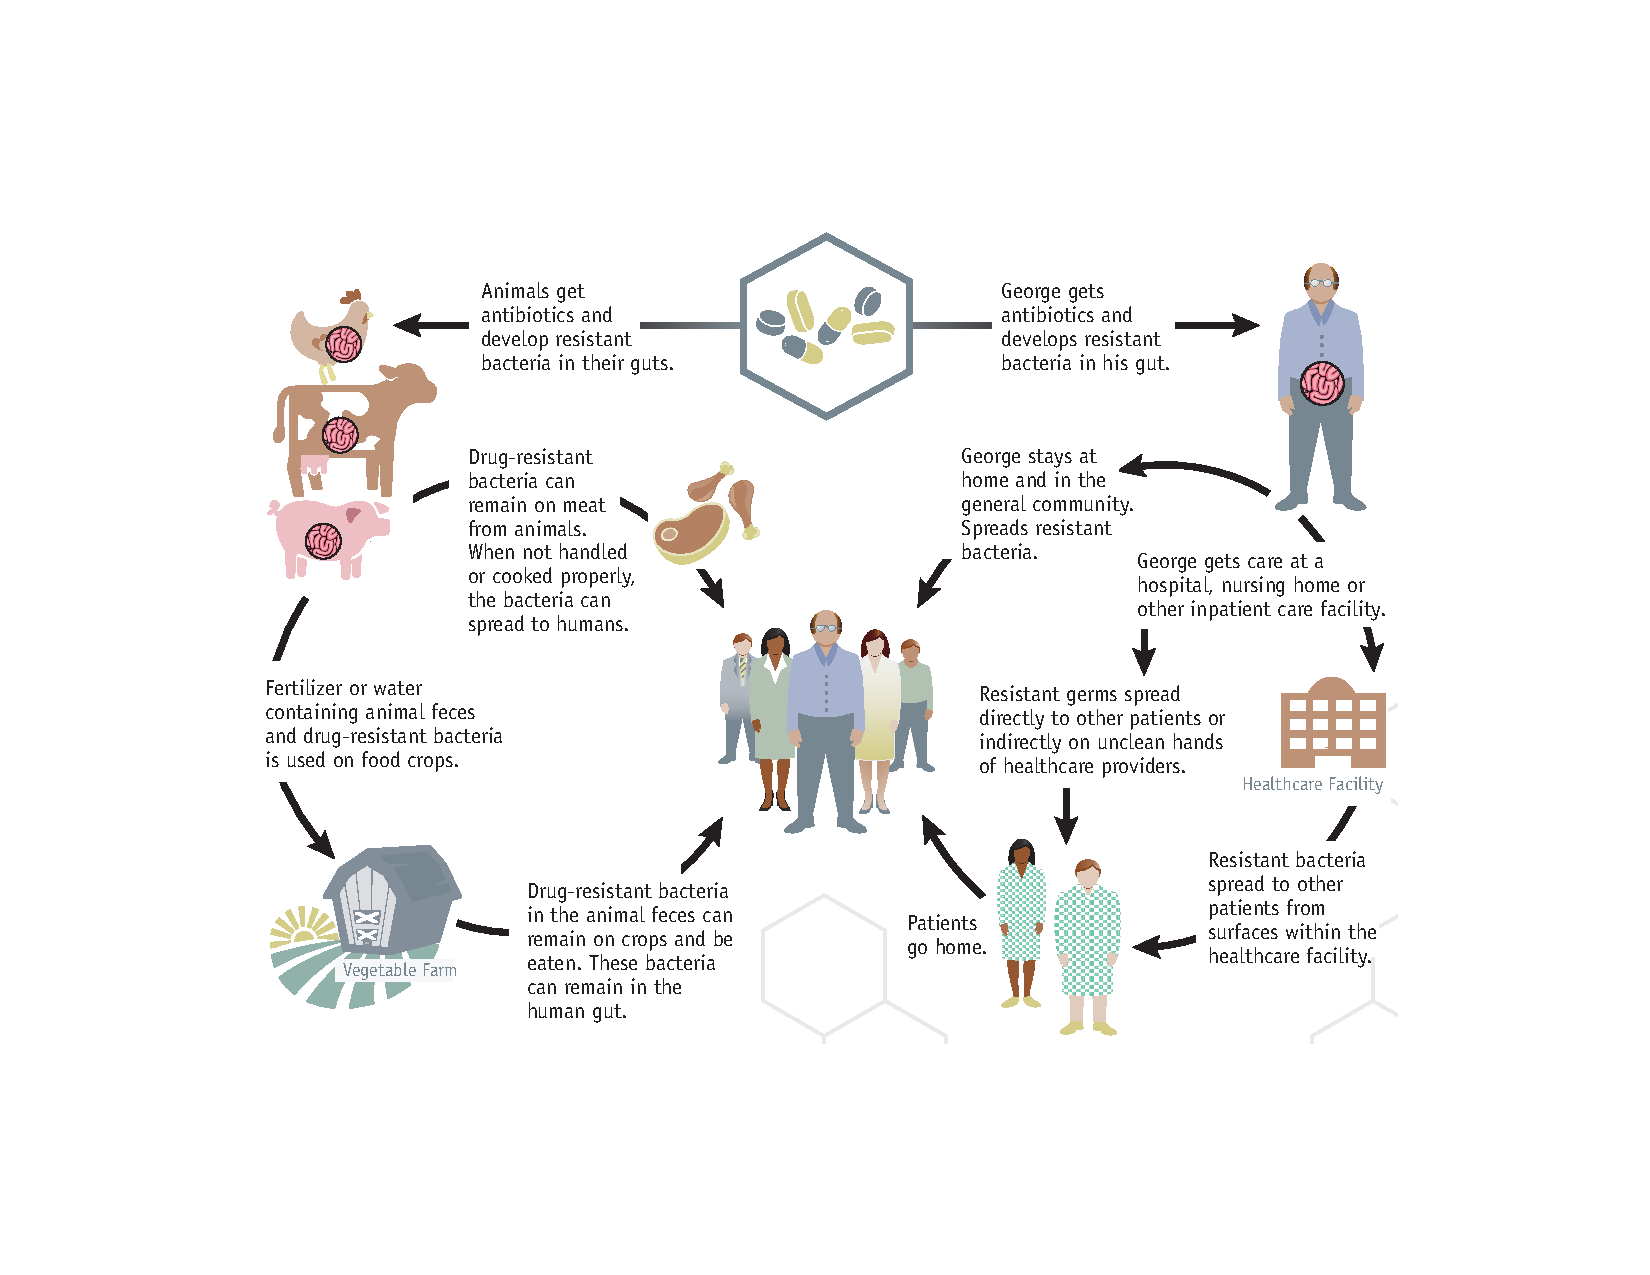
\includegraphics[width=.7\textwidth]{./img/resistant.pdf}
	\caption{Animal food and healthcare system as sources of generating MDROs \cite{resistance}.}
	\label{resistant}
\end{figure}

%In previous section we briefly introduced the HAI prediction problem caused by rare MDROs and discussed its importance. 
 %A study found that 16\% of all HAIs are caused by MDROs \cite{hidron2008antimicrobial}.
In most cases, antibiotic-resistant infections require extended hospital stays, additional follow-up doctor visits, and costly toxic alternatives \cite{amr, resistance}. In 2013, the Centers for Disease Control and Prevention (CDC) published a threat report outlining the top eighteen drug-resistant threats to the U.S. eight of which are healthcare associated with more than 600,000 total occurrences and around 30000 death per year \cite{resistance}. To dive into more scientific details of HAI and also elaborating our data source, in the following, we first introduce the required terminology and then present our dataset. For convenience, Table \ref{tab1} summarizes all of the acronyms and their description. 

% We want to show that they are not studied together. 
{\bf Types of HAI:}
HAIs are categorize by CDC into two broad categories of device-associated infections (DAI) or Surgical-Site Infections (SSI) \cite{mu2011improving, de2006surgical, friedman2007alternative, chiang2014risk}. Primary device-associated infections include Central Line-Associated Bloodstream Infection (CLABSI) \cite{wylie2010risk, noaman2017improving, schoonover2017accurately, herc2017model, parreco2018predicting}, Catheter-Associated Urinary Tract Infection (CAUTI) \cite{grana2015detection, tambyah2004catheter, siddiq2012new}, and Ventilator-Associated Pneumonia (VAP) \cite{froon1998prediction, larsson2017risk, lisboa2008ventilator, kruger2011prognosis, mirsaeidi2009predicting}. Unfortunately, in all of the cited studies, only a single type of HAI is studied in isolation. Based on these studies, many different risk scores have been developed, and preventative measures have been suggested. 

To fully harness the power of data, we suggest to study patients' risks of \emph{all} types of HAIs simultaneously while incorporating the relation of different prediction task in our model. We hypothesized that for a specific infection-causing pathogen, all of the HAIs may share similar risk factors and at the same time each one should have its dedicated important risk factor. For example, one of the main shared risk factors for CDI is recent antibiotic use which is shared among all patients. But patients who had colon surgery have more specific risk factors for developing CDI like length of incision.
We suggest to model the risk of an HAI as a multi-task learning where task are hierarchically related. All HAIs are divided to DAIs and SSIs while DAIs are divided to subtasks based on the relevant device and SSIs are divided based on the place of surgery. Thus, we enrich our dataset with more samples by considering all HIAs together and we are capturing shared and individual per-task risk factors at the same time. 

%Recent studies show reductions in CLABSI incidents due to the advancement in preventative activities while SSI and CAUTI have not experienced the same trend. Different types of HAI can be caused by various organism. 
\begin{table}[]
	\caption{Table of Acronyms and their Descriptions}
	\label{tab1}
	{\footnotesize
		\begin{tabular}{|l|l|r|l|}
			\hline
			\textbf{Name}              & \textbf{Description}                       & \multicolumn{1}{l|}{\textbf{Name}} & \textbf{Description}                               \\ \hline
			\multicolumn{2}{|c|}{\textbf{General Terms}}                            & \multicolumn{2}{c|}{\textbf{Type of HAI}}                                               \\ \hline
			\multicolumn{1}{|r|}{EHR}  & Electronic Health Record                   & CLABSI                             & Central Line-Associated Bloodstream Infection      \\ \hline
			\multicolumn{1}{|r|}{CDC}  & Centers for Disease Control and Prevention & CAUTI                              & Catheter-Associated Urinary Tract Infections       \\ \hline
			\multicolumn{1}{|r|}{NHSN} & National Healthcare Safety Network         & SSI                                & Surgical Site Infection                            \\ \hline
			\multicolumn{1}{|r|}{HAI}  & Healthcare-Associated Infection             & VAP                                & Ventilator-Associated Pneumonia                    \\ \hline
			\multicolumn{1}{|r|}{MDRO} & Multi-Drug Resistant Organism              & \multicolumn{2}{c|}{\textbf{Type of Pathogens}}                                         \\ \hline
			\multicolumn{1}{|r|}{LabID}& Laboratory Identified Event        		& CDI                                & Clostridium difficile, C. diff.                    \\ \hline
			\multicolumn{1}{|r|}{LL}   & Learning Laboratory                        & VRE                                & Vancomycin-resistant Enterococci                   \\ \hline
			\multicolumn{1}{|r|}{TAP}  & Targeted Assessment for Prevention         & MRSA                               & Methicillin-resistant Staphylococcus aureus 	   \\ \hline
			\multicolumn{1}{|r|}{SIR}  & Standardized Infection Ratio               & GNB                                & Gram-negative Bacteria                             \\ \hline
		\end{tabular}
	}
\end{table}


% We provide evidence that they are not examined collectively and more importantly risk prediction is missing for some of them. 
{\bf Types of Pathogens:}
A perpendicular categorization of HAIs is based on the pathogen causing the infection. Although bacteria, fungi, and viruses can cause HAI, four of the most threatening HAI causes are all bacteria and are mostly multi-drug resistant  \cite{resistance, siegel2007management}. In the followings, we briefly introduce each one of the MDROs studied in this proposal:

\begin{itemize}
	\item \underline{Clostridium difficile (CDI):} CDI also known by C. diff bacteria causes life-threatening diarrhea and colitis (an inflammation of the colon). 
	%It was estimated to cause almost half a million infections in the United States in 2011, and 29,000 died within 30 days of the initial diagnosis. 
	Those most at risk are people, especially older adults, who take antibiotics and also get medical care. CDC classifies CDI as an urgent threat and estimates it causes 500,000 infections per year 29,000 of which die within 30 days of the initial diagnosis and 15000 death cases were directly attributed to CDI \cite{resistance}. Although CDI in general is not considered as an MDRO but some variant of it shows resistant to antibiotic  \cite{tenover2012antimicrobial, spigaglia2016recent} and it is monitored by CDC along with other MDROs \cite{cdimdro}. 
	\item \underline{Methicillin-resistant Staphylococcus aureus (MRSA):}  Methicillin-resistant Staphylococcus aureus (MRSA) is a type of staph bacteria that is resistant to certain antibiotics called beta-lactams and has been classified as a serious threat by CDC \cite{resistance}. These antibiotics include methicillin and other more common antibiotics such as oxacillin, penicillin, and amoxicillin. Severe or potentially life-threatening MRSA infections occur most frequently among patients in healthcare settings. By CDC estimate, every year 80400 MRSA infections are happening in the U.S. where more than 11200 of them lead to death \cite{resistance}. 
	\item \underline{Vancomycin-resistant Enterococcus (VRE):} Enterococci cause a range of illnesses, mostly among patients receiving healthcare. Vancomycin-resistant Enterococci are specific types of antimicrobial-resistant bacteria that are resistant to vancomycin, the drug often used to treat infections caused by enterococci. Enterococci are bacteria that are typically present in the human intestines and in the female genital tract and are often found in the environment. Vancomycin-resistant Enterococci infections is considered a serious threat with the death toll of 1300 per year \cite{resistance}.
	\item \underline{Gram-Negative Bacteria (GNB):} GNB is a group of pathogens cause infections including pneumonia, bloodstream infections, wound or SSI, and meningitis in healthcare settings. GNB are resistant to multiple drugs and are increasingly resistant to most available antibiotics. These bacteria have built-in abilities to find new ways to be resistant and can pass along genetic materials that allow other bacteria to become drug-resistant as well \cite{resistance}. Gram-negative infections include those caused by Klebsiella, Acinetobacter, Pseudomonas aeruginosa, and E. coli., as well as many other less common bacteria \cite{gnb}.  
\end{itemize}

{\bf HAI Data Collection:} As a part of CDC the National Healthcare Safety Network (NHSN) is the nation’s most widely used HAI tracking system. Since 2009, infection data has been reported to the NHSN to track the national progress of the reduction of HAIs. For reporting to the NHSN; an infection should be considered as laboratory identified (LabID), i.e., a patient sample should be tested and confirmed positive by laboratory test only (i.e., clinical evaluation of the patient is not required). For LabID events, an infection is considered hospital-onset if the positive specimen is collected on or after the fourth day of admission. NHSN collects hospital-onset LabID infection events to compute different statistics which provides CDC evidence to detect more susceptible healthcare facilities and properly intervene to improve them. 


Standardized Infection Ratio (SIR) is a statistic used to track HAIs over time, at a national, state, or facility level. The SIR is the ratio of the actual number of HAIs at each hospital, to the predicted number of infections. The predicted number is an estimate based on national baseline data, and it is risk adjusted. Risk adjustment takes into account that some hospitals treat sicker patients than others.
Targeted Assessment for Prevention (TAP) is a CDC program that uses data and SIR statistics to identify facilities and units with the most significant burden of excess HAI and target efforts to most efficiently reach prevention goals. TAP guides facilities to customize their interventions to address the identified disproportionate HAIs properly.  
%There have been many model developed ... 

%{\bf Antimicrobial resistance} The result of bacteria changing in ways that reduce or eliminate the effectiveness of drugs, chemicals, or other agents used to cure or prevent infections. Antibiotic resistance is one type of antimicrobial resistance.

%{\bf :} It is known that some hospitals and some units are more susceptible to MDROs and therefore have higher number of HAI cases. TAP is a method developed by the CDC to use data for action to prevent HAIs. The TAP strategy targets healthcare facilities and specific units within facilities with a burden of
%HAIs to address infection prevention gaps.
%
%{\bf :} 


%Methicillin-resistant Staphylococcus aureus (MRSA): A type of staph bacteria that is resistant to many antibiotics. In this report, the MRSA data include all laboratory identified hospital-onset MRSA bacteremia (bloodstream infections) reported to the National Healthcare Safety Network from all inpatient locations in
%the facility.



%bacteria that cause life-threatening diarrhea. Often,
%C. difficile infections occur in hospitalized or recently hospitalized
%patients. In this report, the C. difficile data include all laboratory
%identified hospital-onset infections reported to the National
%Healthcare Safety Network from all inpatient locations in the
%facility, with the exception of the neonatal intensive care units and
%well-baby locations.


%MRSA remains an important cause of HAIs, and it is endemic in most hospitals in the U.S. In
%addition to increasing the total burden of S. aureus infection, health care-associated MRSA
%infections are associated with increased morbidity and mortality compared with infections
%caused by methicillin-susceptible strains. Furthermore, MRSA has emerged as an important
%cause of infection in the community. Fifty-nine percent of all purulent skin infections
%evaluated in U.S. emergency departments are caused by MRSA. MRSA infections, both
%health care- and community-associated, are generally caused by a very limited number of
%strains, suggesting that most cases result from direct or indirect person-to-person
%transmission of MRSA.

% These infections lead to the loss of tens of thousands lives and cost the U.S. health care system billions of dollars each year. Though many risk factors are well-known for some types of HAI, particularly central-catheter-associated bloodstream infections, other types of HAIs continue to burden patients and health care system with ? costs. Is has been estimated by the Centers for Disease Control and Prevention (CDC) that 1.7 million health care-associated infections occur per year over U.S. hi

%Catheter-associated urinary tract infection (CAUTI): A urinary tract
%infection (UTI) is an infection involving any part of the urinary
%system, including urethra, bladder, ureters, and kidney. When a
%urinary catheter is not put in correctly, not kept clean, or left in a
%patient for too long, germs can travel through the catheter and
%infect the bladder and kidneys. In this report, the CAUTI data
%include all infections reported to the National Healthcare Safety
%Network from all applicable locations, including intensive care
%units and wards.
%
%Central line-associated bloodstream infection (CLABSI): When
%a tube is placed in a large vein and not put in correctly or kept
%clean, it can become a way for germs to enter the body and cause
%deadly infections in the blood. In this report, the CLABSI data
%include all infections reported to the National Healthcare Safety
%Network from all applicable locations, including intensive care
%units, neonatal intensive care unit, and wards.

%Healthcare-associated infection (HAI): An infection patients can
%get while receiving medical treatment in hospitals, outpatient
%clinics, nursing homes, and other facilities where people receive
%care
%
%Surgical site infection (SSI): When germs get into an area where
%surgery is or was performed, patients can get a surgical site
%infection. Sometimes these infections involve only the skin. Other
%SSIs can involve tissues under the skin, organs, or implanted
%material (an object or material inserted or grafted into the body,
%such as prosthetic joints).

%Ventilator-associated events (VAE): A ventilator is a machine used
%to help a patient breathe by giving oxygen through a tube placed
%in a patient’s mouth or nose, or through a hole in the front of the
%neck. An infection, such as pneumonia, may occur if germs enter a
%patient through the tube.


{\bf IDEA4PS Dataset:}
In 2015, the OSU was awarded a four-year program project grant from the Agency of Healthcare Research and Quality to establish The Institute for the Design of Environments Aligned for Patient Safety (IDEA4PS). This grant is being used to identify and explore how feedback of information can be used to inform the development of robust practices that lead to improved patient safety. As a part of IDEA4PS temporal patient's data has been collected to conduct surveillance of healthcare-acquired infections in real time and to provide clinicians with actionable information.

We will leverage IDEA4PS data to train our ML system, DEALER and integrate it to the OSU hospital system. {\color{red} add data stat here. }
%This learning lab integrates system engineering, design, human factors, organizational behavior, evaluation, and data analysis to explore the way feedback of information is incorporated into the adaptation of work systems to enhance patient safety. The intent is to frame how all kinds of data, both those currently collected and newly acquired, are leveraged to actionable information and linked to patient outcomes.


% What are the possible interventions
{\bf Interventions:}
Although it seems that for the patients with higher risk of infection the care team should carry out the most effective interventions, in reality, this is not the best measure. Serious interventions are usually more difficult to tolerate by the patient, and they are of more significant cost for the healthcare system. Besides, for the specific intervention of antibiotic administration the rise of drug-resistant organisms urge us to use antibiotics only if they are absolutely necessary and by following strict ``antibiotic stewardship'' guidelines.

The epidemiology of emergent MDROs in health care settings must be monitored to allow for appropriate adaptations to current infection control interventions, including antimicrobial prophylaxis, isolation strategies, and screening strategies. Vaccines are also a powerful way to prevent thousands of infections and deaths that occur each year for diseases such as influenza and hepatitis. Currently, there are eight vaccines licensed in the U.S. that target pathogens that can be acquired in health care settings. The appropriate use of these lifesaving interventions needs to be defined.
A successful ML system should take into account the range of possible intervention and based on its confidence about the predicted outcome suggest a proper intervention.


% What are the specific questions that we want to address?
% Why are these questions challenging?
\subsection{Motivating Problems and Challenges}
{\noindent \bf Problem 1:} Given a set of MDROs where some of them are extremely rare, we want to leverage patients static (demographic, sex, etc.) and temporal features (vitals, lab results, etc.) to predict the desired outcomes. Examples of the desired outcome include, but not limited to, timely prediction of the occurrence of a specific MDRO incident (discrete outcome) or prediction of time to infection (continuous outcome).

{\noindent \bf Problem 2:} Given a task of predicting an extremely rare HAI, incorporate the domain expert knowledge about the involved risk factors into the ML system and provide an interpretable answer that suggests which collection of risk factors are affecting the prediction outcome the most.

{\noindent \bf Problem 3:} Given a heterogeneous source of data like hospitals and units therein where the whole environment that data has been gathered is different and also collected features are not exactly similar, tailor the prediction for each hospital or unit while leveraging the similarities between each environment.

We describe below some of the key technical challenges involved in addressing these problems and how we plan to solve them:

\underline{Prediction of rare events:} As reported by many studies, HAIs affect less than 10\% of the hospital admitted patients which makes any collected dataset highly imbalanced. Among all HAIs some of them like C. diff. are rare while others like VRE are extremely rare. Highly imbalanced data induce unique challenges for learning algorithms. We propose to ...

\underline{Structure of data:} We propose to study admitted patients to the OSU hospital system which consists of x main hospitals each of which has between y to z units. A naive algorithm would put together all of the patients' data and analyze that as a single dataset. However, a more sophisticated approach will take into account the hierarchical structure that the hospitals induce on patients which is extremely important in the context of infectious diseases. Another important structure is the relation of different MDRO, exploiting similarities and differences between MDROs will potentially improve the outcome of prediction algorithms.

\underline{Timely Prediction}: Data shows that the longer a patient stays in the hospital, the more it is probable to acquire an HAI. Therefore using patients longitudinal data is essential for any practical algorithm. Also, evaluation of any method should consider the length of time window between flagging a patient as high risk and the actual infection happening.

\underline{Interpretability}: Since different outcomes of the risk prediction algorithm require the care team to carry out different preventative measures, e.g., isolation, or administration of prophylaxis, the algorithm should explain its decisions. Clinicians are hesitant to incorporate weakly evaluated black-box ML algorithms into their practice. Therefore, interpretability should be addressed in every level of the proposed ML system.

\underline{Missing data:}  The widespread prevalence of missing data in electronic health records presents a significant challenge for any ML algorithm. Different causes of missing data in the EHR data may introduce unintentional bias, and therefore any level of the proposed ML system should be robust to missing data.

\underline{Hidden factors:} Many known risk factors for HAIs are hard to measure and therefore are unknown to the algorithm. Factors like cleaning protocols, quality of care, and the presence of colonized carrier are important hidden risk factors that make the prediction task more complicated.  For example, it is known that the C. diff. spores can persist on environmental surfaces, and therefore the role of environmental cleaning is likely to be significant. For MRSA, it is widely held that the primary reservoir for transmission in the health care setting is infected or colonized patients and that patient-to-patient transmission occurs indirectly via transient carriage by health care personnel or through shared equipment that is contaminated.

%In 2005, there were an estimated 94,000 invasive MRSA infections in the United States, which were
%associated with nearly 18,000 deaths. Of these invasive infections, 86% were associated with
%health care delivery, but two-thirds of these HAIs had their onset outside the hospital setting.
%Recent data suggest that between 2005 and 2008, rates of invasive health care-associated
%MRSA infection decreased.12
%Although the optimal strategy for preventing and controlling health care-associated MRSA
%has not been fully determined, it is likely that successful control requires a multifaceted
%approach that may vary according to the individual characteristics of a health care facility, as
%outlined in the CDC guidance document Management of Multidrug-resistant Organisms in
%Healthcare Facilities, 2006.
%Additionally, there is a growing recognition that the focus of
%MRSA prevention on individual health care facilities needs to be broadened to incorporate
%entire geographic regions.




\subsection{Technical Approach}
{\bf Notation:} 
How do we come up with the labels from the data? 

- The simplest way to label is to consider data points only at the admission time or post surgery time. 
- More complicated way of labeling is to label every instance one time window before the incident as one. 


- Homogeneous feature MTL is the first case

Notation:
	MTL is the general framework of handling our problem:Define tasks, homo-features, ...
	Why do we elevate something as a task? (When to share)
		- Domain expert: previously people have considered HAI types separately. 
			- Human expert is the one deciding in the literature.
			- Cross-validation is computationally intensive. 
		- We gain more flexibility and interpretability. 
	
Fast optimization method for solving any of these. 
	
P1: Focus on one facility but predict multiple MDRO infections. 
Talk about the history of multi task learning: parameter, feature ?, instance based sharing. 

	- Time to event (listen to Kevin's comment)
	- 

P2: 
a) Focus on multiple facilities but predict one MDRO: MTL for single MDRO heterogeneous
b) Focus on multiple facilities but predict multiple MDRO: MTL with multiple output MDRO heterogeneous
 - Here we go beyond the known MTL literature
 
P3: Intervention



\subsubsection{Problem 1: Multi-output Prediction of Extremely Rare Event: Multi-task Learning}
\subsubsection{Problem 2: Multi-output Prediction of Extremely Rare Event: Hierarchical Samples and Transfer Learning}
\subsubsection{Problem 3: }

Considerable hospital resources are dedicated to minimizing the number of methicillin-resistant Staphylococcus aureus (MRSA) infections. One tool that is commonly used to achieve this goal is surveillance for MRSA colonization. This process is costly, and false-positive test results lead to isolation of individuals who do not carry MRSA. The performance of this technique would improve if patients who are at high risk of colonization could be readily targeted.




Data sharing, data enrichment, multi task learning, sparse task differences, imbalanced classification.

\noindent {\bf Problem 1:} A few questions/commentspotential directions:
\begin{itemize}
\item For patient specific prediction, consider/contrast with {\em Cox proportional hazards model} (CPHM), and other forms of {\em survival analysis}. Here, 'survival' refers to staying un-infected.
\item For a group based model, consider/contrast with {\em multiple instance learning} (MIL). The goal here is to characterize if any one individual in a cohort will have MDR infection. The cohorts can be formed based on (static and temporal) patient covariates, say by clustering, and/orbased on physical location, e.g., a certain unit in a clinic. MIL have had mixed success in the literature, so we have to be careful about what we propose.
\end{itemize}

\noindent {\bf Problem 2:} How do we plan to make things interpretable? Couple of possible approaches:
\begin{itemize}
\item Importance of individual features: One can assess individual feature importance in nonlinear models, including random forests, gradient boosted trees, and deep nets, by an ablation study, i.e., by studying predictive accuracy by leaving each feature out. 
\item Importance of sub-groups of features: Doing ablation study with sub-groups naively leads to an exponential blow-up in computation. One can consider doing PCA regression, sufficient dimensionality reduction, or Shapley value regression in such settings.
\end{itemize}
Few considerations in the current context: 
\begin{itemize}
\item Can such feature importance be done efficiently? 
\item How does one take into account the fact that the target events are rare? 
\item How does one handle the small sample regime, so feature importance is assessed at the population level, not because it helps overfit on the training set?
\item How do the proposed approaches relate to sparse methods? Shall we use sparse methods instead?
\item How do the proposed approaches related to frequent pattern mining for prediction problems?
\end{itemize}

\noindent {\bf Problem 3:} Since we will be combining data from multiple clinics, the samples are going to be disjoint (similar to our current data-sharing model), but the features will have some shared and some unique covariates (different from our current model).



\subsection{System Evaluation}
Evaluation of any method should consider the length of time window between flagging a patient as high risk and the actual infection happening.

\subsection{Comparison of Our Approach to Related Work}

\subsection{Community Outreach and Education}

\subsection{Results from Prior NSF Support}

\subsection{Collaboration Plan}

\noindent
\emph{\underline{Name of PI}}: NSF-Program (Award Number) ``Title of the Project'' (\$AMOUNT, PERIOD OF SUPPORT).
{\bf Publications:} List of publications resulting from the NSF award. A complete bibliographic citation for each
publication must be provided either in this section or in the References Cited section of the proposal); if
none, state: ``No publications were produced under this award.'' {\bf Research Products:} evidence of research products
and their availability, including, but not limited to: data, publications, samples, physical collections, software,
and models, as described in any Data Management Plan.
